\documentclass[a4paper,11pt]{article}
\usepackage[margin=24mm]{geometry}
\usepackage{fontspec,unicode-math,booktabs,graphicx,amsmath,hyperref}
\setmainfont{STIXGeneral}\setmathfont{STIX Two Math}
\hypersetup{hidelinks}
\setlength{\emergencystretch}{2em}\setlength{\parindent}{0pt}\setlength{\parskip}{5pt}
\title{Rank contraction: complete written costs}
\author{Human Compression project}
\date{Private numerical candidate; distinct review pending}
\begin{document}\maketitle\raggedright
The original is Brooksbank--Leemans, \emph{Rank reduction of string C-group
representations}, arXiv:1812.01055v2, 3 May 2019. The accepted scope contains
22 source clauses and 20 proof contexts. This comparison measures the complete
source manuscript and the complete common paper and application, with no
free overlap with earlier Topic B theory. It makes no new mathematical or
source-credit claim.

\section*{Written papers}
The primary unit is the number of non-whitespace characters in the complete
raw PDF extraction, normalized to NFC. Titles, author blocks, running furniture,
references and the application’s references-only final page are included.
\begin{center}\begin{tabular}{@{}lrr@{}}\toprule Complete document & Pages & Characters\\\midrule
Original L037 & 6 & 15,530\\
Whole common theory $U$ & 3 & 6,937\\
Application $A$ & 5 & 10,555\\
Written replacement $U+A$ & 8 & 17,492\\
Complete printed program & 1 & 2,925\\\bottomrule\end{tabular}\end{center}
The combined written comparison is
\[\frac{c(L037)}{c(U)+c(A)}=\frac{15530}{17492}=0.887834.\]
A value below one means that the replacement is longer in this coordinate.
Here the complete written replacement has 1,962 more characters than the source.
\begin{center}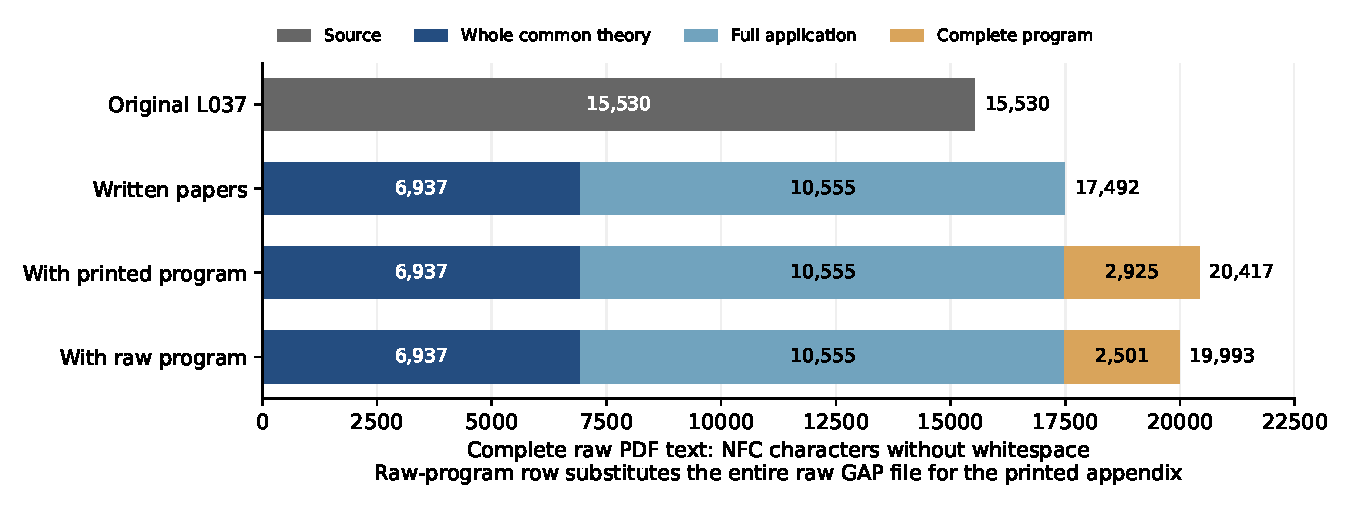
\includegraphics[width=\linewidth]{costs.pdf}\end{center}
\newpage
\section*{Including the complete program}
The GAP file \texttt{check\_examples.g} is required for the displayed matrix and
three literal $A_{11}$ examples and includes doubled-edge validation. The uniform
rank-contraction theorem and its infinite families do not depend on its output.
The complete printed appendix costs 2,925 characters; the whole raw program
costs 2,501 characters. These are alternatives:
\[
\frac{c(L037)}{c(U)+c(A)+c(\mathrm{printed\ program})}=\frac{15530}{20417}=0.760641,
\]
\[
\frac{c(L037)}{c(U)+c(A)+c(\mathrm{raw\ program})}=\frac{15530}{19993}=0.776772.
\]
Neither row combines the printed and raw versions. No line or diagnostic part
is pruned from the whole file.

\section*{After acquiring the theory and program}
Only after acquiring \emph{all} of $U$ and the complete declared program is the
conditional application comparison
\[\frac{c(L037)}{c(A)}=\frac{15530}{10555}=1.471341.\]
The prior acquisition costs are $6,937+2,925=9,862$ characters using the printed
program, or $6,937+2,501=9,438$ using the raw alternative. This conditional ratio
does not assert that the complete replacement is shorter.

\section*{Separate costs and limits}
The complete operational driver has 6,950 raw bytes and 6,114 primary
non-whitespace characters. The complete Lean file has 1,727 raw bytes and 1,280
primary characters. Its four declarations are scoped group-algebra facts;
they do not formalize the full contraction theorem, its classical seeds or the
source. These files are separately inventoried and are not silently included in
the program rows. The mathematical GAP file has 2,680 raw bytes.

The end criterion and stated highest-rank classical constructions, orthogonal
identifications and the prior $A_{11}$ exhaustion remain retained inputs. Their
full proof costs, historical software and full formalization costs are unknown,
not zero. Conjecture 5.1 remains an open research target; no answer or question
credit is claimed.

The source’s three diagrams contain 264 XYCIRC glyph events. Every variant
retains their literal extracted \texttt{/c16} through \texttt{/c23} strings.
Those strings are not a complete measurement of the drawn graphs. Formula and
graph layout costs also remain unknown; no full-visible-text or intrinsic
mathematical-complexity claim is made.

The numerical author separately reviewed the accepted inputs but is the author
of these new calculations, not their independent numerical reviewer. Publication
requires a distinct review. No GAP or Lean computation was repeated for these
numbers.
\newpage
\section*{Metric and extraction sensitivity}
All 30 coordinates use the same whole-document boundary. The five units are
computed under NFC and NFKC. ``Printed'' and ``Raw'' include the corresponding
whole program representation; ``Conditional'' assumes the full prior acquisition
specified above. The JSON and CSV files retain all 120 exact fractions; the table
rounds only the display.

{\small \subsection*{Complete raw extraction}\begin{tabular}{@{}llrrrr@{}}\toprule Unit & Form & Written & Printed & Raw & Conditional\\\midrule Whitespace tokens & NFC & 0.978970 & 0.924299 & 0.941117 & 1.643425 \\
Alphanumeric runs & NFC & 0.994126 & 0.850194 & 0.864808 & 1.656139 \\
Non-space characters & NFC & 0.887834 & 0.760641 & 0.776772 & 1.471341 \\
Collapsed characters & NFC & 0.904151 & 0.787669 & 0.803984 & 1.501794 \\
Collapsed UTF-8 bytes & NFC & 0.872465 & 0.767703 & 0.782502 & 1.485940 \\
Whitespace tokens & NFKC & 0.982913 & 0.928022 & 0.944908 & 1.650044 \\
Alphanumeric runs & NFKC & 0.994126 & 0.850194 & 0.864808 & 1.656139 \\
Non-space characters & NFKC & 0.889181 & 0.761993 & 0.778127 & 1.475428 \\
Collapsed characters & NFKC & 0.905936 & 0.789377 & 0.805705 & 1.506315 \\
Collapsed UTF-8 bytes & NFKC & 0.921638 & 0.805353 & 0.821683 & 1.537991 \\\bottomrule\end{tabular}
\subsection*{Exact furniture removed}\begin{tabular}{@{}llrrrr@{}}\toprule Unit & Form & Written & Printed & Raw & Conditional\\\midrule Whitespace tokens & NFC & 0.971549 & 0.917413 & 0.933907 & 1.631137 \\
Alphanumeric runs & NFC & 0.986085 & 0.843249 & 0.857575 & 1.642889 \\
Non-space characters & NFC & 0.877145 & 0.751470 & 0.767376 & 1.453649 \\
Collapsed characters & NFC & 0.894022 & 0.778833 & 0.794910 & 1.485012 \\
Collapsed UTF-8 bytes & NFC & 0.863096 & 0.759454 & 0.774044 & 1.470049 \\
Whitespace tokens & NFKC & 0.975501 & 0.921144 & 0.937706 & 1.637771 \\
Alphanumeric runs & NFKC & 0.986085 & 0.843249 & 0.857575 & 1.642889 \\
Non-space characters & NFKC & 0.878511 & 0.752838 & 0.768747 & 1.457749 \\
Collapsed characters & NFKC & 0.895824 & 0.780554 & 0.796645 & 1.489544 \\
Collapsed UTF-8 bytes & NFKC & 0.911761 & 0.796712 & 0.812812 & 1.521556 \\\bottomrule\end{tabular}
\subsection*{Furniture removed and eight bracket events calibrated}\begin{tabular}{@{}llrrrr@{}}\toprule Unit & Form & Written & Printed & Raw & Conditional\\\midrule Whitespace tokens & NFC & 0.971549 & 0.917413 & 0.933907 & 1.631137 \\
Alphanumeric runs & NFC & 0.986085 & 0.843249 & 0.857575 & 1.642889 \\
Non-space characters & NFC & 0.877145 & 0.751470 & 0.767376 & 1.453649 \\
Collapsed characters & NFC & 0.894022 & 0.778833 & 0.794910 & 1.485012 \\
Collapsed UTF-8 bytes & NFC & 0.863096 & 0.759454 & 0.774044 & 1.470049 \\
Whitespace tokens & NFKC & 0.975501 & 0.921144 & 0.937706 & 1.637771 \\
Alphanumeric runs & NFKC & 0.986085 & 0.843249 & 0.857575 & 1.642889 \\
Non-space characters & NFKC & 0.878511 & 0.752838 & 0.768747 & 1.457749 \\
Collapsed characters & NFKC & 0.895824 & 0.780554 & 0.796645 & 1.489544 \\
Collapsed UTF-8 bytes & NFKC & 0.911761 & 0.796712 & 0.812812 & 1.521556 \\\bottomrule\end{tabular}}

Exact furniture removal deletes only isolated page numbers and repeated running
headers. It keeps the source’s arXiv banner. The calibrated sensitivity replaces
eight font- and occurrence-bound square-bracket components by their visible
Unicode counterparts, retaining one component per event. Here that changes text
hashes but none of the five metric counts. Printed hyphens remain literal.
\end{document}
